\section{SimpIL: The language}
A precise definition of dynamic taint analysis or forward symbolic execution must target a specific language: we use SimpIL, a Simple Intermediate Language. Although the language is simple, it is powerful enough to express typical languages as varied as Java and assembly code. Indeed, the language is representative of internal representations used by compilers for a variety of programming languages. A program in this language consists of a sequence of numbered statements. Statements in our language consist of assignments, assertions, jumps, and conditional jumps.

I don't want to bore you with the details of the operational semantic, but spending a few minutes talking about the grammar is necessary. Expressions are side-effect free, and we use \texttt{$\lozenge$b} to represent typical binary operators, e.g., addition, subtraction, etc. Similarly, \texttt{$\lozenge$u} represents unary operators such as logical negation. The statement \texttt{get\_input(src)} returns input from source \texttt{src}. For simplicity, we consider only expressions (constants, variables, etc.) that evaluate to 32-bit integer values.

\begin{figure}[ht!]
	\caption{SimpIL Grammar}
	\centering
	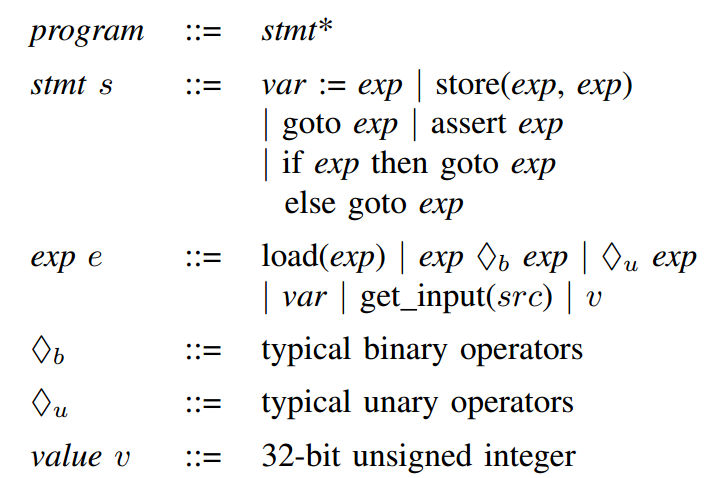
\includegraphics[width=0.7\textwidth]{SimpILBN}
\end{figure}

We do not include some high-level language constructs such as functions or scopes for simplicity reasons. This omission does not fundamentally limit the capability of our language or our results. Adding such constructs is trivial, and we can do both by compiling missing high-level language constructs down to the language or by adding them in a native way. Furthermore we don't really care about types: designing a sound and strong type system is possible, but we are not interested in that: remember that the dynamic analysis is dynamic, while a sound type checking should be static.

